\chapter{ Технологический раздел}
\label{cha:technological}

    В данном разделе будут выбраны средства реализации ПО и представлен листинг кода. 

    \section{Средства реализации}
        В данной работе используется язык программирования golang \cite{go}, так как
        он позволяет написать программу в относительно малый срок за счёт
        встроенных средств распараллеливания и взаимодействия потоков, таких как gorutine и сhannels \cite{go-concurrency}. 
        В качестве среды разработки использовалась Visual Studio Code \cite{visual-studio-code}.

        Для получения текущего времени была использована функция Now() модуля time. 
        Для упрощения работы с ней используется обёртка getTime, 
        код которой представлен в листинге \ref{lst:getTime}.

        \begin{lstlisting}[language=go, label=lst:getTime, caption=Функция получения текущего времени]
func getTime() string {
    return time.Now().Format("15:04:05.99999999")
}
        \end{lstlisting}

    \section{Листинг программы}
        Ниже представлены листинги кода системы:
        \begin{enumerate}
            \item генерации значений (листинг \ref{lst:generate});
            \item декоратора этапа (листинг \ref{lst:action});
            \item реализация ступеней конвейера (листинг \ref{lst:action:step});
            \item реализация точки входа в программу (листинг \ref{lst:main}).
        \end{enumerate}
        
        \begin{lstlisting}[language=go, label=lst:generate, caption=Реализация генерации значений]
func generate(n int) <-chan int {
    queue := make(chan int)

    go func() {
        defer close(queue)

        for i := 0; i < n; i++ {
            value := rand.Intn(100)
            fmt.Print("time: ", getTime(), " send: ", value, "\n")
            queue <- value
        }
    }()

    return queue
}
        \end{lstlisting}

        \begin{lstlisting}[language=go, label=lst:action, caption=Реализация декоратора этапа конвейера]
type actionFunc func(int) int

func action(source <-chan int, name string, f actionFunc) <-chan int {
    result := make(chan int)

    go func() {
        defer close(result)

        for arg := range source {
            fmt.Print("time: ", getTime(), " in ", name, ": ", arg, "\n")
            value := f(arg)
            fmt.Print("time: ", getTime(), " out ", name, ": ", value, "\n")
            result <- value
        }
    }()

    return result
}
        \end{lstlisting}

        \begin{lstlisting}[language=go, label=lst:action:step, caption=Реализация ступеней конвейера]
func stepA(arg int) int {
    time.Sleep(100)
    return arg * arg
}

func stepB(arg int) int {
    time.Sleep(200)
    return arg * arg
}

func stepC(arg int) int {
    time.Sleep(150)
    return arg * arg
}
        \end{lstlisting}
    
        \begin{lstlisting}[language=go, label=lst:main, caption=Реализация точки входа в программу]
func main() {
    var count int
    fmt.Print("Enter generate count: ")
    _, err := fmt.Scanf("%d", &count)
    if err != nil {
        fmt.Println(err)
        os.Exit(-1)
    }

    var queue = generate(count)
    queue = action(queue, "A", stepA)
    queue = action(queue, "B", stepB)
    queue = action(queue, "C", stepC)

    for res := range queue {
        fmt.Print("time: ", getTime(), " res: ", res, "\n")
    }
}
        \end{lstlisting}
        
    \section{Тестирование}
        На рисунке \ref{png:testing:result} представлен результат работы программы.
        Из времени поступления и отправки значения из разных этапов можно заключить, 
        что одновременно обрабываются разные элементы на разных этапах,
        следовательно программа работает корректно.

        \begin{figure}[h!]
            \centering
            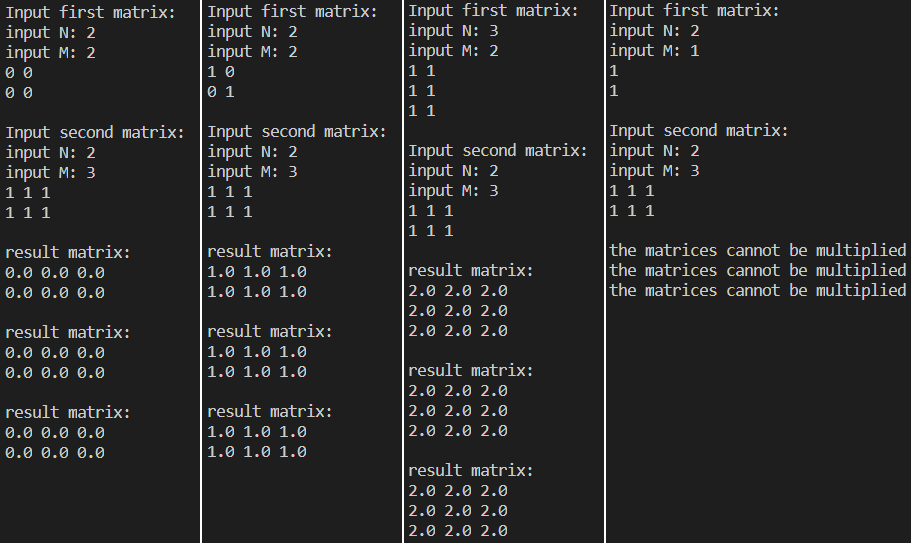
\includegraphics[scale=0.9]{testing.png}
            \caption{Результаты тестирования алгоритмов.}
            \label{png:testing:result}
        \end{figure}
\newpage